\documentclass[mathserif,professionalfont,hyperref={pdfpagelabels=false}]{beamer}
\usepackage{pxfonts} 
%\usepackage{eulervm}
\usepackage[english]{babel}
\usepackage{calc}
\usepackage[absolute,overlay]{textpos}
\mode<presentation>{\usetheme{tud}}
%\usepackage{subcaption}
\usepackage{tcolorbox}
\usepackage{tikz}
\usetikzlibrary{positioning,arrows}
\usepackage[utf8x]{inputenc}
\usepackage{scalefnt}
\usetikzlibrary{decorations.markings}
\usetikzlibrary{shapes,snakes}
\usetikzlibrary{shapes.geometric}
\usetikzlibrary{fit}					
\usetikzlibrary{backgrounds}
\usetikzlibrary{positioning}
\usetikzlibrary{arrows}
\usepackage{pgffor}
\usepackage{amsmath,amssymb,mathrsfs}
\usepackage{amsthm}
\usepackage{color}
\usepackage{wasysym}
\usepackage{pdfpages}
\usepackage{paralist}
\usepackage{framed}
\usepackage{fancybox} %kaders
\usepackage{pifont}
\usepackage{pgfplots}
\usepackage{listofsymbols}
\usepackage{multirow}
\usepackage{appendixnumberbeamer}
\usepackage[scaled]{helvet}
\usepackage[round]{natbib}
\tikzstyle{every picture}+=[remember picture]
\tikzstyle{na} = [baseline=-.5ex]
\usepgfplotslibrary{units}

\title[]{\normalsize{Understanding flow slides in flood defences}}
\institute[]{}
\author[]{Lisa Wobbes}
\date[\today]{\today}

\definecolor{blueM}{rgb}{0.4, 0.6, 0.8}


\begin{document}
%titel---------------------------------------------------------------------------------------------------------------------------------------------------------------------------
{
%\usebackgroundtemplate{\includegraphics[width=\paperwidth,height=\paperheight]{logos}}%
%\setbeamertemplate{footline}{\usebeamertemplate*{minimal footline}}
\frame{\titlepage}
}

%-------------------------------------------------------------------------------------------------------------------------------------------------------------------------------
\begin{frame}{Recap}
Last time:
\begin{itemize}
\item Accuracy vibrating bar with MATLAB and Fortran
\item Courses 
\end{itemize}
\pause
 Work in progress:
\begin{itemize}
\item Accuracy tests for oedometer
\item Reading papers on liquefaction:
\begin{itemize}
\item Byrne and Eldridge, A three parameter dilatant elastic stress-strain model for sand (1982)
\item Byrne et al., Numerical modeling of liquefaction and comparison with centrifuge test (2004)
\end{itemize}
\item Started writing first year report 
\end{itemize}
\end{frame}
%-------------------------------------------------------------------------------------------------------------------------------------------------------------------------------
\begin{frame}{Outline}
\begin{itemize}
\item Accuracy vibrating string revisited
\item Accuracy oedometer with Fortran implementation
\item Validation of 2-phase FEM
\item Long term model
\item Boston
\item Short term planning
\end{itemize}
\end{frame}

%-------------------------------------------------------------------------------------------------------------------------------------------------------------------------------

\begin{frame}{Vibrating bar}
  \begin{minipage}{\linewidth}
      \centering
      \begin{minipage}{0.45\linewidth}
              \definecolor{darkred}{cmyk}{0,0.9,0.9,0.2}
\definecolor{darkblue}{cmyk}{0.9,0.5,0.1,0.2}
\tikzset{
mystyle1/.style={
  rectangle,
  inner sep=0.05pt,
  text width=1mm,
  fill=black
  }
}

\tikzset{
mystyle2/.style={
  circle,
  inner sep=0.1pt,
  text width=2mm,
  fill=red!80
  }
}
\tikzstyle{myarrows}=[line width=0.4mm,draw=darkred,postaction={draw, line width=0.4mm, shorten >=3mm, -}]
\begin{figure}[H]
\centering
\begin{tikzpicture}[scale=0.48]
 %structure
 \draw[fill=black!25] (0.5,2) rectangle (6.5,2.55);
 \draw[fill=darkblue] (-0.3,3.5) rectangle (0.5,1);
%initial velocity
%\foreach \i in {1,2,3,4,5}
%{
%        \pgfmathsetmacro{\z}{0.5 + (6/5)*\i};
%        \pgfmathsetmacro{\y}{2.275};
%        \pgfmathsetmacro{\l}{1.1*sin((175*\z)/12)};
%        \draw[myarrows] (\z,\y) -- (\z+\l,\y);
%	\draw[->, ultra thick,darkred] (\z+1.01*\l,\y) -- (\z+1.05*\l,\y);
%}
%\draw (7.2,3.2) node {$v_0$};

\draw (7.2,3.2) node {$v_0$};
\draw[arrows={-latex'}, ultra thick,darkred] (6,2.275) -- (6.5+1.05*2,2.275);
%coordinate
\draw[->, thick] (-0.3,0.2)--(8.9,0.2);
\draw (8.5, -0.4) node {$x$};
 %coordinates
 \draw[thick] (0.5, 0.05)--(0.5,0.35);
 \draw (0.5,-0.4) node {0};
 \draw[thick] (6.5, 0.05)--(6.5,0.35);
 \draw (6.5,-0.4) node {$L$};
\end{tikzpicture}
\end{figure}
      \end{minipage}
      \hspace{0.01\linewidth}
      \begin{minipage}{0.45\linewidth}
         \begin{align}\nonumber
&\frac{\partial^2 u}{\partial t^2} = \frac{E}{\rho}\frac{\partial^2 u}{\partial x^2} \\ \nonumber
&\mbox{Boundary conditions: } \\  \nonumber
& u(0,t) = 0\\ \nonumber
& \frac{\partial u}{\partial x}(L,t) = 0\\  \nonumber
&\mbox{Initial conditions:}\\  \nonumber
& u(x,0) = 0\\ \nonumber
& \frac{\partial u}{\partial t}(x,0) = v_0\sin \left( \frac{\pi x}{2L} \right)
\end{align} 
      \end{minipage}
  \end{minipage}
\end{frame}



%-------------------------------------------------------------------------------------------------------------------------------------------------------------------------------
\begin{frame}{Accuracy vibrating bar: Fortran}
\definecolor{RYB3}{RGB}{31, 148, 254}
\begin{center}
\begin{figure}
\begin{tikzpicture}[scale=0.9]
\begin{axis}[
        xlabel=number of elements,
        xmode=log,
        log basis x={2},
        xtick = {4,8,16,32,64, 128},
        xticklabels={4,8,16,32,64, 128},
        ylabel=$\log_2$(RMS error), 
	y unit=m,
        ymode=log,
        log basis y={2},
	ytick = {0.03125,0.0078125, 0.001953125, 4.8828125e-04, 1.220703125e-04,3.0517578125e-05, 7.62939453125e-06,1.9073486328125e-06, 4.768371582031250e-007},
%         ytick = {2^{-9},2e-11,2e-13,2e-15,2e-15,2e-17,2e-19},
         yticklabels={-5,-7,-9,-11,-13,-15,-17,-19,-21}
]
\addplot[color=blue,mark=square*] coordinates { 
  (4,  3.8010e-04) 
  (8,  9.5225e-05)
  (16, 2.4213e-05)
  (32, 8.4138e-06)
  (64, 2.1019e-06)
  (128, 3.7553e-07)
  };
  

\addplot[color=red, mark=*] coordinates { 
  (4,  2.5677e-03) 
  (8,  8.1946 e-04)
  (16, 2.2593e-04)
  (32, 7.1407e-05)
  (64, 2.0510e-05)
  (128, 3.4562e-06) 
  };
  
\addplot[color=black,mark=triangle*] coordinates { 
  (4,  1.4566e-03) 
  (8,  4.1500e-04)
  (16,1.0620e-04)
  (32,2.89536e-05)
  (64, 9.5836e-06)
  (128,4.9559e-06) 
  };  

\addplot[color=RYB3,mark=x] coordinates { 
(4, 1.6974e-03)
(8, 4.9514e-04)
(16, 1.2917e-04)
(32, 3.7018e-05)
(64, 1.1473e-05)
(128,4.3115e-06)
};
\legend{FEM, MPM(1), MPM(4), MPM(8)} 
\end{axis}
%\end{semilogyaxis} 
\end{tikzpicture}
\end{figure}
\end{center}
\end{frame}

%-------------------------------------------------------------------------------------------------------------------------------------------------------------------------------
\begin{frame}{Accuracy vibrating bar: Fortan}
\centering
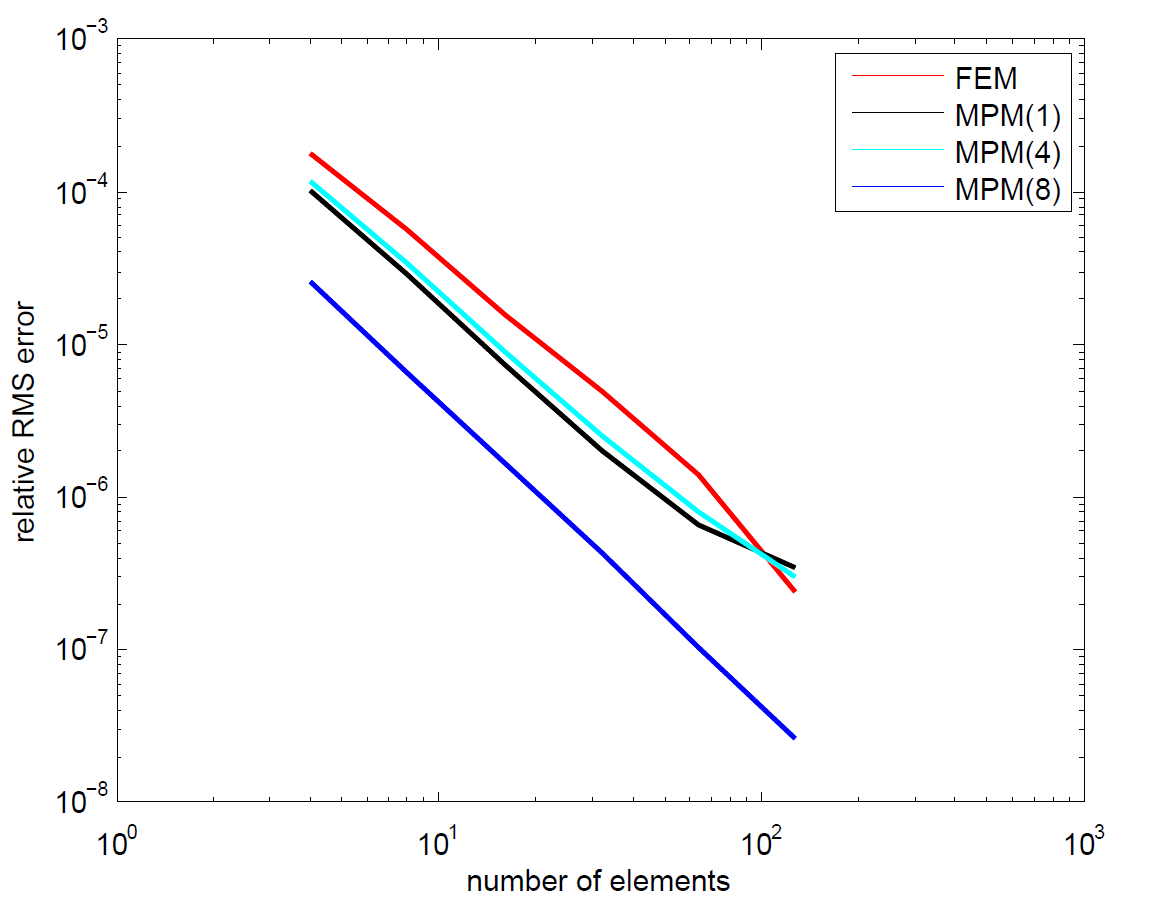
\includegraphics[width=0.7\paperwidth,height=0.7\paperheight]{images/accuracy_vib_bar}
\end{frame}

%-------------------------------------------------------------------------------------------------------------------------------------------------------------------------------
\begin{frame}{Oedometer (small deformations)}
  \begin{minipage}{\linewidth}
      \centering
      \begin{minipage}{0.45\linewidth}
\definecolor{soil}{cmyk}{0,0.2,0.6,0.2}
\definecolor{darkred}{cmyk}{0,0.9,0.9,0.2}
\tikzset{
mystyle1/.style={
  rectangle,
  inner sep=0.05pt,
  text width=1mm,
  fill=black
  }
}

\tikzset{
mystyle2/.style={
  circle,
  inner sep=0.1pt,
  text width=2mm,
  fill=red!80
  }
}
\tikzstyle{myarrows}=[line width=0.4mm,arrows={-latex'},darkred, postaction={draw, line width=0.4mm, shorten >=3mm, -}]
\begin{figure}[h]
\centering
\begin{tikzpicture}
 %structure
 \draw[fill=black] (0.4,2.2) rectangle (2.6,-1.1);
 \draw[fill=soil] (0.5,2) rectangle (2.5,-1);
 \draw[fill=black!25] (0.5,2) rectangle (2.5,2.35);
 \draw (1.5, 0.5) node {soil};

 %load
 \draw[myarrows] (0.7,3) -- (0.7,2.35);
 \draw[myarrows] (1.5,3) -- (1.5,2.35);
 \draw[myarrows] (2.3,3) -- (2.3,2.35);
%\draw[arrows={-latex'}, ultra thick,darkred] (0.7,2.35) -- (0.7,2.34);
%\draw[arrows={-latex'}, ultra thick,darkred] (1.5,2.35) -- (1.5,2.34);
%\draw[arrows={-latex'}, ultra thick,darkred] (2.3,2.35) -- (2.3,2.34);
 \draw (1.55,3.3) node {$p_0$};
%coordinate axis
\draw[->, thick] (-1,-1.2)--(-1,3.3);
\draw (-1.3, 3.1) node {$y$};
 %coordinates
\draw[thick] (-1.1,2)--(-0.9,2); 
\draw (-1.3,2) node {$H$};
\draw[thick] (-1.1,-1)--(-0.9,-1);
\draw (-1.3,-1) node {0};
\end{tikzpicture}
\end{figure}
      \end{minipage}
      \hspace{0.01\linewidth}
      \begin{minipage}{0.45\linewidth}
         \begin{align}\nonumber
&\frac{\partial^2 u}{\partial t^2} = \frac{E}{\rho} \frac{\partial^2 u}{\partial^2 y} -g \\ \nonumber
&\mbox{Boundary conditions: } \\  \nonumber
& u(0,t) = 0\\ \nonumber
& \frac{\partial u}{\partial y}(H,t) = \frac{p_0}{E} = 0\\ \nonumber
&\mbox{Initial conditions:}\\  \nonumber
& u(y,0) = 0\\ \nonumber
& \frac{\partial u}{\partial t}(y,0) = 0
\end{align} 
      \end{minipage}
  \end{minipage}
\end{frame}
%-------------------------------------------------------------------------------------------------------------------------------------------------------------------------------
\begin{frame}{Accuracy oedometer}
\begin{itemize}
\item MATLAB: lack of convergence with FEM and MPM
\pause
\item Fortran: lack of convergence with FEM and MPM\\
\pause
Approaches used with FEM: 
\begin{itemize}
\item Absolute RMS error
\item Relative RMS error
\item Richardson (node on top)
\item Absolute RMS error with a gradual increase of the gravitational force
\end{itemize}
\end{itemize}
\end{frame}
%-------------------------------------------------------------------------------------------------------------------------------------------------------------------------------
\begin{frame}{2-phase FEM: consolidation}
\centering
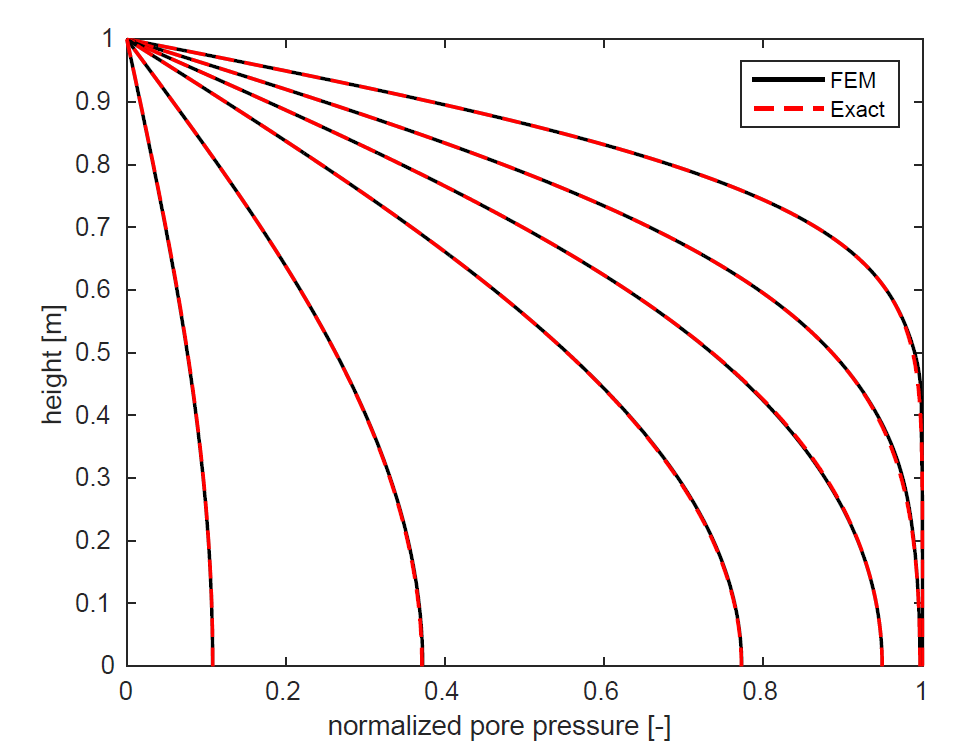
\includegraphics[width=0.7\paperwidth,height=0.7\paperheight]{images/consolidation}
\end{frame}
%-------------------------------------------------------------------------------------------------------------------------------------------------------------------------------
\begin{frame}{2-phase FEM: one-dimensional wave propagation}
\centering
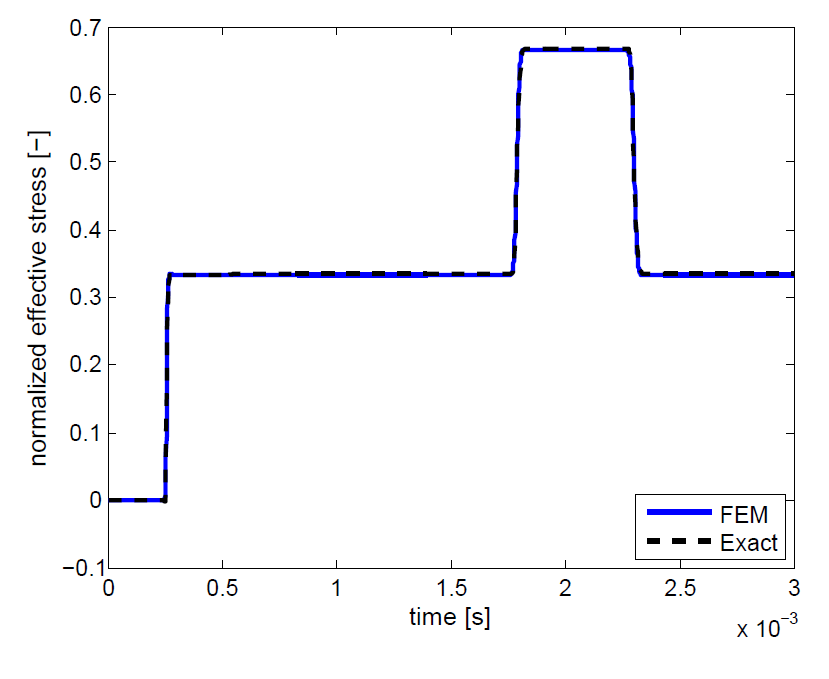
\includegraphics[width=0.8\paperwidth,height=0.8\paperheight]{images/efs_1Dwave_prop}
\end{frame}
%-------------------------------------------------------------------------------------------------------------------------------------------------------------------------------
\begin{frame}{2-phase FEM: one-dimensional wave propagation}
\centering
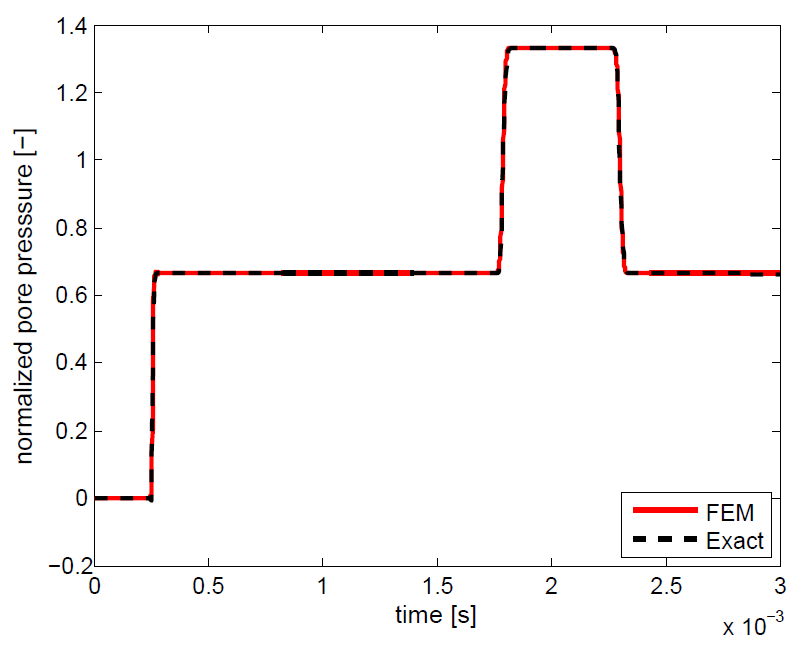
\includegraphics[width=0.8\paperwidth,height=0.8\paperheight]{images/pp_1Dwave_prop}
\end{frame}
%-------------------------------------------------------------------------------------------------------------------------------------------------------------------------------



\begin{frame}{``Long" term planning}
\begin{itemize}
\item Within FEM replace elastic material model by Drucker-Prager model
\pause
\item Within FEM replace Drucker-Prager model by Mohr-Coulomb model (?)
\pause
\item Integrate FEM with models suggested by Byrne (Stolle)
\pause
\item Switch to MPM for large deformations
\end{itemize}
\end{frame}


%-------------------------------------------------------------------------------------------------------------------------------------------------------------------------------
\begin{frame}{``Short" term planning/Work in progress}
\begin{itemize}
\item 2-phase MPM implementation in MATLAB
\item Reading Byrne et al., Numerical modeling of liquefaction and comparison with centrifuge test (2004)
\pause
\item Appointment with Prof. Stolle
\item Study Drucker-Prager model
\item Write out the implementation of Drucker-Prager 
\end{itemize}
\end{frame}

%-------------------------------------------------------------------------------------------------------------------------------------------------------------------------------
\begin{frame}{Boston}
\begin{itemize}
\item Submitted abstract
\item Trying to find financial support
\end{itemize}
\end{frame}

%-------------------------------------------------------------------------------------------------------------------------------------------------------------------------------
%-------------------------------------------------------------------------------------------------------------------------------------------------------------------------------
%-------------------------------------------------------------------------------------------------------------------------------------------------------------------------------

\appendix

\begin{frame}{Settings: vibrating bar}
\begin{table}[h]
\centering
\begin{tabular}{l | c c c}
 & Symbol & Value & Unit \\
\hline
Length& $L$ & 25 & m\\
Tension& $E$ & $ 100$ & Pa\\
Density & $\rho$ & $1$ & kg/m$^3$\\
Maximum velocity & $v_0$ & 0.1 & m/s\\
%Load & $p_0$ & $-5\cdot 10^3$ & Pa\\
%Gravitational acceleration & $g$ & 9.81 & m/s$^2$\\ 
Time step & $\Delta t$ &$ 1 \cdot10^{-3}$ & s\\
Measurement time & $t$ & 0.5 & s\\
%PPC$^2$ & & 4 & \\
\end{tabular}
\end{table}
\end{frame}

%-------------------------------------------------------------------------------------------------------------------------------------------------------------------------------

\begin{frame}{Accuracy vibrating bar: MATLAB}
\definecolor{RYB3}{RGB}{31, 148, 254}
\begin{overlayarea}{\textwidth}{6cm}
\begin{center}
\only<1>{
\begin{figure}
\begin{tikzpicture}[scale=0.9]
\begin{axis}[
        xlabel=number of elements,
        xmode=log,
        log basis x={2},
        xtick = {4,8,16,32,64},
        xticklabels={4,8,16,32,64},
        ylabel=$\log_2$(RMS error), 
	y unit=m,
        ymode=log,
        log basis y={2},
	ytick = {0.001953125, 4.8828125e-04, 1.220703125e-04,3.0517578125e-05, 7.62939453125e-06,1.9073486328125e-06, 4.768371582031250e-007},
%         ytick = {2^{-9},2e-11,2e-13,2e-15,2e-15,2e-17,2e-19},
         yticklabels={-9,-11,-13,-15,-17,-19,-21}
]
\addplot[color=blue,mark=square*] coordinates { 
  (4,  5.3698e-04) 
  (8,  1.3456e-04)
  (16, 3.3657e-05)
  (32, 8.4138e-06)
  (64, 2.1019e-06)
  };
  
\addplot[color=red, mark=*] coordinates { 
  (4,  1.2918e-03) 
  (8,  3.2595 e-04)
  (16, 8.1795e-05)
  (32, 2.0632e-05)
  (64, 5.4969e-06)
  };
  
\addplot[color=black,mark=triangle*] coordinates { 
  (4,  1.0374e-03) 
  (8,  2.6167e-04)
  (16, 6.5694e-05)
  (32, 1.6625e-05)
  (64, 4.5505e-06)
  };  


\addplot[color=RYB3,mark=x] coordinates { 
(4,9.667486e-04)
(8,2.438081e-04)
(16,6.121801e-05)
(32,1.551265e-05)
(64,4.252232e-06)
};
\legend{FEM, MPM(1), MPM(4), MPM(8)} 
\end{axis}
%\end{semilogyaxis} 
\end{tikzpicture}
\end{figure}
}
\only<2>{
\begin{figure}
\begin{tikzpicture}[scale=0.9]
\begin{axis}[
        xlabel=number of elements,
        xmode=log,
        log basis x={2},
        xtick = {4,8,16,32,64, 128},
        xticklabels={4,8,16,32,64, 128},
        ylabel=$\log_2$(RMS error), 
	y unit=m,
        ymode=log,
        log basis y={2},
	ytick = {0.001953125, 4.8828125e-04, 1.220703125e-04,3.0517578125e-05, 7.62939453125e-06,1.9073486328125e-06, 4.768371582031250e-007},
%         ytick = {2^{-9},2e-11,2e-13,2e-15,2e-15,2e-17,2e-19},
         yticklabels={-9,-11,-13,-15,-17,-19,-21}
]
\addplot[color=blue,mark=square*] coordinates { 
  (4,  5.3698e-04) 
  (8,  1.3456e-04)
  (16, 3.3657e-05)
  (32, 8.4138e-06)
  (64, 2.1019e-06)
  (128,5.2381e-07)
  };
  
\addplot[color=red, mark=*] coordinates { 
  (4,  1.2918e-03) 
  (8,  3.2595 e-04)
  (16, 8.1795e-05)
  (32, 2.0632e-05)
  (64, 5.4969e-06)
  (128, 2.1502e-06) 
  };
  
\addplot[color=black,mark=triangle*] coordinates { 
  (4,  1.0374e-03) 
  (8,  2.6167e-04)
  (16, 6.5694e-05)
  (32, 1.6625e-05)
  (64, 4.5505e-06)
  (128, 1.9769e-06) 
  };  

\addplot[color=RYB3,mark=x] coordinates { 
(4,9.667486e-04)
(8,2.438081e-04)
(16,6.121801e-05)
(32,1.551265e-05)
(64,4.252232e-06)
(128,3.928155e-06)
};
\legend{FEM, MPM(1), MPM(4), MPM(8)} 
\end{axis}
%\end{semilogyaxis} 
\end{tikzpicture}
\end{figure}
}
\end{center}
\end{overlayarea}
\end{frame}


%------------------------------------------------------------------------------------------------------------------
\begin{frame}{Accuracy vibrating bar: Fortran}
\definecolor{RYB3}{RGB}{31, 148, 254}
\begin{overlayarea}{\textwidth}{6cm}
\begin{center}
\only<1>{
\begin{figure}
\begin{tikzpicture}[scale=0.9]
\begin{axis}[
        xlabel=number of elements,
        xmode=log,
        log basis x={2},
        xtick = {4,8,16,32,64},
        xticklabels={4,8,16,32,64},
        ylabel=$\log_2$(RMS error), 
	y unit=m,
        ymode=log,
        log basis y={2},
	ytick = {0.03125,0.0078125, 0.001953125, 4.8828125e-04, 1.220703125e-04,3.0517578125e-05, 7.62939453125e-06,1.9073486328125e-06, 4.768371582031250e-007},
%         ytick = {2^{-9},2e-11,2e-13,2e-15,2e-15,2e-17,2e-19},
         yticklabels={-5,-7,-9,-11,-13,-15,-17,-19,-21}
]

\addplot[color=blue,mark=square*] coordinates { 
  (4,  3.8010e-04) 
  (8,  9.5225e-05)
  (16, 2.4213e-05)
  (32, 8.4138e-06)
  (64, 2.1019e-06)
  };
  
  
\addplot[color=red, mark=*] coordinates { 
  (4,  2.5677e-03) 
  (8,  8.1946 e-04)
  (16, 2.2593e-04)
  (32, 6.2733e-05)
  (64, 1.5129e-05)
  };
  
\addplot[color=black,mark=triangle*] coordinates { 
  (4,  1.4566e-03) 
  (8,  4.1500e-04)
  (16,1.0620e-04)
  (32,2.89536e-05)
  (64, 9.5836e-06)
  };  

\addplot[color=RYB3,mark=x] coordinates { 
(4, 1.6974e-03)
(8, 4.9514e-04)
(16, 1.2917e-04)
(32, 3.7018e-05)
(64, 1.1473e-05)
};
\legend{FEM, MPM(1), MPM(4), MPM(8)} 
\end{axis}
%\end{semilogyaxis} 
\end{tikzpicture}
\end{figure}
}
\only<2>{
\begin{figure}
\begin{tikzpicture}[scale=0.9]
\begin{axis}[
        xlabel=number of elements,
        xmode=log,
        log basis x={2},
        xtick = {4,8,16,32,64, 128},
        xticklabels={4,8,16,32,64, 128},
        ylabel=$\log_2$(RMS error), 
	y unit=m,
        ymode=log,
        log basis y={2},
	ytick = {0.03125,0.0078125, 0.001953125, 4.8828125e-04, 1.220703125e-04,3.0517578125e-05, 7.62939453125e-06,1.9073486328125e-06, 4.768371582031250e-007},
%         ytick = {2^{-9},2e-11,2e-13,2e-15,2e-15,2e-17,2e-19},
         yticklabels={-5,-7,-9,-11,-13,-15,-17,-19,-21}
]
\addplot[color=blue,mark=square*] coordinates { 
  (4,  3.8010e-04) 
  (8,  9.5225e-05)
  (16, 2.4213e-05)
  (32, 8.4138e-06)
  (64, 2.1019e-06)
  (128, 3.7553e-07)
  };
  

\addplot[color=red, mark=*] coordinates { 
  (4,  2.5677e-03) 
  (8,  8.1946 e-04)
  (16, 2.2593e-04)
  (32, 7.1407e-05)
  (64, 2.0510e-05)
  (128, 3.4562e-06) 
  };
  
\addplot[color=black,mark=triangle*] coordinates { 
  (4,  1.4566e-03) 
  (8,  4.1500e-04)
  (16,1.0620e-04)
  (32,2.89536e-05)
  (64, 9.5836e-06)
  (128,4.9559e-06) 
  };  

\addplot[color=RYB3,mark=x] coordinates { 
(4, 1.6974e-03)
(8, 4.9514e-04)
(16, 1.2917e-04)
(32, 3.7018e-05)
(64, 1.1473e-05)
(128,4.3115e-06)
};
\legend{FEM, MPM(1), MPM(4), MPM(8)} 
\end{axis}
%\end{semilogyaxis} 
\end{tikzpicture}
\end{figure}
}
\end{center}
\end{overlayarea}
\end{frame}

%-------------------------------------------------------------------------------------------------------------------------------------------------------------------------------
\end{document}